\chapter{Cold-Atom Electron and Ion Source}\label{chapter:setup}

The \gls{caeis} at the University of Melbourne is a source of low temperature electrons or rubidium ions with promising potential as a alternative charge particle source.
The \gls{caeis} works by carefully ionising rubidium atoms trapped in a \gls{mot} in order to generate a low temperature plasma which can then be accelerated to form a particle beam.
The apparatus described here is reaching the end of it's useful life, greater understanding of the limitations imposed by this implementation of a \gls{caeis} and the already impressive developments achieved with this source have paved the way for the next generation of \gls{caeis} which is not compatible with the apparatus.
Numerous doctoral students have worked on this system and the design and construction details can be found in their theses~\cite{sheludko_shaped_2010,bell_cold_2011,saliba_cold_2011,mcculloch_generation_2013,murphy_measurement_2017,rory_thesis}.

This chapter provides an overview of the \gls{caeis} and some of the investigations into source stability, source current and beam optimisation.

\section{Description}
In order to generate electrons and ions the University of Melbourne \gls{caeis} began by trapping and cooling atoms in a \gls{mot} that was loaded from a Zeeman slower.
The optical and magnetic trapping fields were then extinguised and the ground-state atoms carefully ionised using a combination of a red excitation laser and a blue ionisation laser.
The charged particles are accelerated by a static electric produced by the accelerators electrodes, one polarity accelerating ions towards the detector and the other electrons.

When the source is acting as an electron source the it is essential to turn off the \gls{mot} and Zeeman slower magnetic fields before ionisation due to the significant deviation that the fields cause to the electron trajectories.
Ion trajectories are not adversly affected if the fields are left on due to the much higher ion mass.

{\color{red}Figure showing setup. Perhaps Fig 2.1 from Rory's thesis.}

\subsection{Rubidium Oven}
The source begins with an effusive Rubidium oven with a long heated collimation tube.
Typically effusive ovens are wasteful with large numbers of atoms lost into a large solid angles however this experimented makes use of a long heated collimation tube to collect and re-emit atoms that were initially emitted at high angles.
These atoms are re-emitted back to the reservoir or into the collimated atom beam leaving the collimation tube.
A brief schematic of the oven can be found to the left in Figure~\ref{figure:zeemanoven} and more detail on the design, operation, and performance of the oven can be found in References~\cite{bell_slow_2010} and \cite{bell_cold_2011}.

\begin{figure}
    \center
    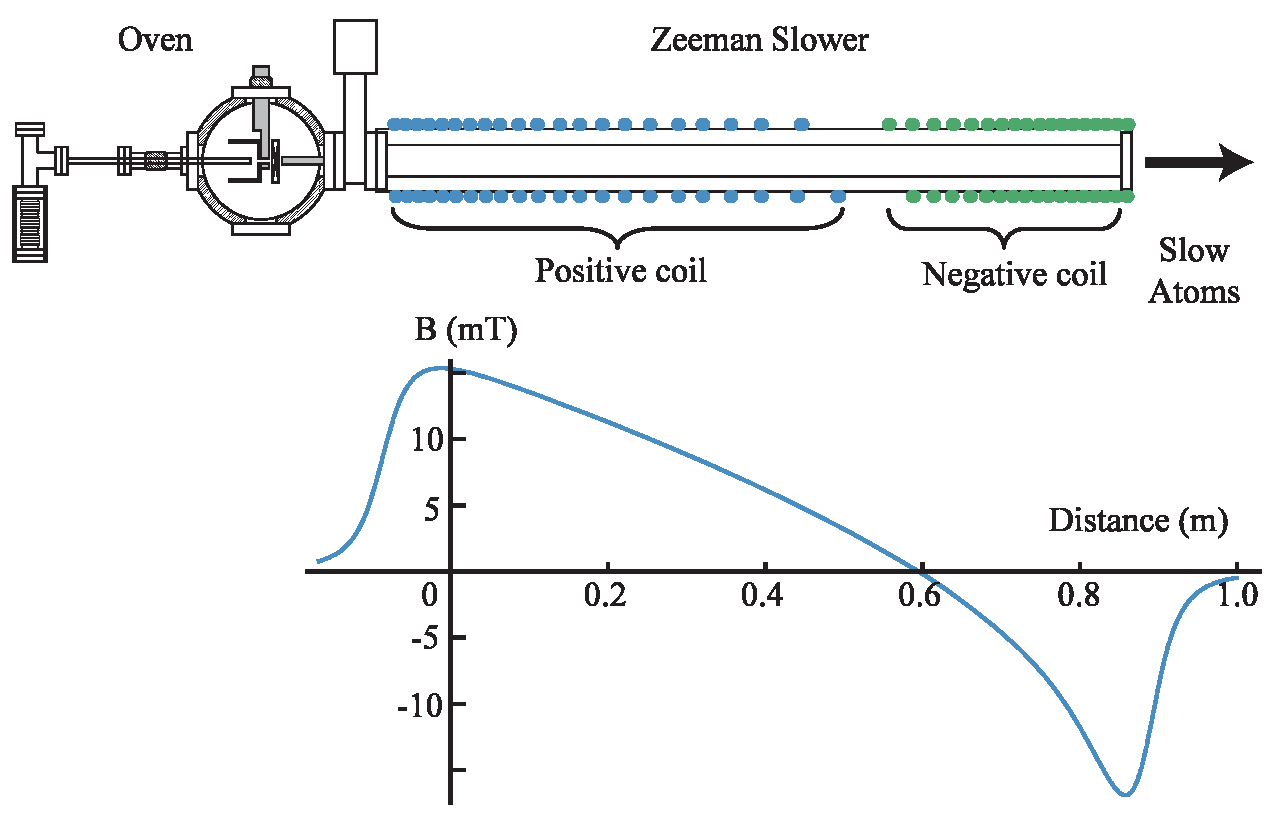
\includegraphics[width=130mm]{part2/Figs/ZeemanOven.pdf}
    \caption{A schematic of the rubidium atom source. Atomic vapour from the oven is directed into the Zeeman slower where a laser detuned from the atomic resonance, in combination with a tapered magnetic coil, with a magnetic field as shown, slows the thermal atoms.}
    \label{figure:zeemanoven}
\end{figure}

\subsection{Zeeman Slower}
Following the oven is the tapered pitch Zeeman slower which slows atoms down so that they can be captured by the trapping fields of \gls{mot}~\cite{bell_slow_2010}.
Zeeman slowers operate by using a laser red-detuned from resonance to slow the atoms down however as the atoms slow the conditions for resonance change due to the changing Doppler shift.
The solution to this quandrary used here is a tapered magnetic coil to apply a magnetic field to shift the atomic resonance such that a particular velocity class of atoms remains resonant with the light field, and thus is slowed, along the length of the Zeeman slower.
A schematic of the Zeeman slower with along with the magnetic field produced by the tapered coil is shown in Figure~\ref{figure:zeemanoven}.

When extracting electrons from the \gls{mot} the magnetic coil must be turned off to prevent disruptions to the electron trajectory.

\subsection{Magneto-Optic Trap}
The \gls{mot} serves to trap the atoms for ionisation and to cool them to lower temperatures.

\subsection{Two-Colour Ionisation}

\subsubsection{Beam Shaping}

\subsubsection{Ultrafast Laser}

\subsection{Accelerator}

\subsection{Electron Optics}

\subsection{Sample Management}

\subsubsection{Sample Holder}

\subsubsection{Samples}

\subsection{Detector}

\section{Properties}

The primary advantage of \glspl{caeis} over alternative sources is the low transverse temperature of the particles produced.
Electrons produced from the sources can have temperatures as low as \unit[10]{K} which is extrememly low when compared to other electron sources such as photocathode sources (\unit[$10^3$-$10^4$]{K}~\cite{claessens_ultracold_2005}).

Cold

High coherence

Low emittance

Shaping

Reversal of space charge expansion

Ions or electrons

Applicable to any atom that can be trapped.


\section{How it works}

\label{section:two_stage_ionisation}
\label{section:excess_energy}
\label{section:pulse_blaster}

\section{Current Limitations}

\section{Pulsed vs Continuous}

\subsection{Oven Temperature to Electron Count}

\section{Stability}\label{section:stability}

\section{Source Characterisation}

\subsection{Astigmatism}

\subsubsection{Quadrupole Correction}\label{section:quadrupole}

\subsection{Emittance Measurements}

\subsection{Streaked emittance}

\subsection{Coherence}

\subsection{Noise characterisation}

\section{Future Ideal source}